% !TeX program = pdflatex
%==============================================================================
%  Aula 08 --- Métricas para Classificação
%  VERSÃO DO ALUNO: texto para leitura autônoma, fora da sala.
%  (O roteiro de sala é "08 Metricas para Classificacao.tex".)
%==============================================================================
\documentclass[11pt,a4paper]{article}
\usepackage[aluno]{../../recursos/latex/estilo-notas}

\title{}
\date{}

\begin{document}
\cabecalhoaula{08}{Métricas para Classificação}{AME §7.4 e cap.~9; ISLP §4.4--4.5}

%==============================================================================
\section*{O que você vai aprender}
%==============================================================================
Ao final desta aula você deve ser capaz de:
\begin{itemize}[leftmargin=1.4cm]
  \item explicar por que a acurácia pode ser uma medida enganosa, quando uma das
        classes é rara ou quando os dois tipos de erro têm custos diferentes;
  \item construir a \textbf{matriz de confusão}, definir sensibilidade,
        especificidade, precisão, valor preditivo negativo e $F_1$ como estimativas
        de probabilidades, e escrever o risco em termos das taxas de erro de cada
        classe;
  \item deduzir o \textbf{corte ótimo} de um classificador \emph{plug-in} sob uma
        perda assimétrica;
  \item definir a \textbf{curva ROC}, interpretar a \textbf{AUC} e reconhecer quando
        a curva precisão--revocação informa mais;
  \item comparar as estratégias para dados desbalanceados: mover o corte, reponderar
        e reamostrar;
  \item distinguir \emph{classificar bem} de \emph{estimar bem probabilidades} e
        avaliar a calibração com regras de pontuação próprias.
\end{itemize}

\noindent
A Aula~07 terminou com um aviso: a acurácia pode enganar. Esta aula desenvolve esse
aviso a partir de uma pergunta simples:

\begin{center}\itshape
  numa população em que $1\%$ das pessoas tem certa doença, um teste que declara\\
  todo mundo saudável acerta $99\%$ das vezes. Ele é um bom teste?
\end{center}

\noindent
Não é: ele não encontra doente nenhum. A acurácia, porém, não registra isso, porque
soma num único número dois erros de natureza muito diferente. O que segue constrói
medidas que separam esses erros e mostra como escolher entre elas conforme a
pergunta que se quer responder.

%==============================================================================
\section{Por que a acurácia não basta}
%==============================================================================
Considere a classificação binária, com $Y\in\{0,1\}$, e um classificador $g$. A
Aula~07 avaliou $g$ pelo risco $0$--$1$,
\[
  \risco(g)=\Prob\big(g(\X)\neq Y\big),
\]
cujo complemento, $1-\risco(g)$, é a \textbf{acurácia}. Esse critério trata todo erro
como igual, e há duas situações frequentes em que isso não serve.
\begin{itemize}[leftmargin=1.4cm]
  \item \emph{Custos assimétricos.} Num exame de rastreamento, deixar de detectar um
        doente (um \emph{falso negativo}) costuma ser muito mais grave que mandar um
        saudável para um exame confirmatório (um \emph{falso positivo}). O risco
        $0$--$1$ dá aos dois o mesmo peso.
  \item \emph{Uma classe rara.} Se $\pi_1=\Prob(Y=1)$ é pequena, o classificador
        trivial $g\equiv0$ tem risco $\pi_1$ e acurácia $1-\pi_1$, alta, sem acertar
        positivo nenhum. Mais que isso: se as covariáveis informam pouco sobre $Y$,
        pode acontecer de $\Prob(Y=1\mid\X=\x)<1/2$ para todo $\x$, e então o próprio
        classificador de Bayes é $g\equiv0$ ([AME] §9.1). Os métodos que aproximam o
        classificador de Bayes passam a aproximar o classificador trivial.
\end{itemize}

\begin{atencao}
O desbalanceamento, sozinho, não é um defeito do problema. Se os dois erros custam o
mesmo, o classificador de Bayes minimiza exatamente o que interessa, a probabilidade
de erro, por mais rara que seja uma das classes. A dificuldade aparece quando os
custos diferem: o classificador de Bayes pesa os dois erros igualmente e deixa de
ser o classificador desejado. As técnicas das Seções~\ref{sec:custos}
a~\ref{sec:desb} são maneiras de levar esses custos em conta.
\end{atencao}

%==============================================================================
\section{Matriz de confusão e métricas}
%==============================================================================
Para avaliar um classificador $g$ já construído, usa-se uma \emph{amostra de teste}
$(\X_1,Y_1),\dots,(\X_m,Y_m)$: observações i.i.d.\ com a distribuição de $(\X,Y)$ e
independentes dos dados usados para construir $g$. A classe $Y=1$ é chamada de
\emph{positiva}; em geral, é a classe de interesse, como o doente ou a fraude.
Cruzar o que $g$ prediz com o valor verdadeiro produz quatro contagens,
\[
  \text{VP}=\#\{i : g(\X_i)=1,\ Y_i=1\},\qquad
  \text{FP}=\#\{i : g(\X_i)=1,\ Y_i=0\},
\]
\[
  \text{FN}=\#\{i : g(\X_i)=0,\ Y_i=1\},\qquad
  \text{VN}=\#\{i : g(\X_i)=0,\ Y_i=0\},
\]
os verdadeiros e falsos positivos e negativos, que se organizam na \textbf{matriz de
confusão} da Figura~\ref{fig:confusao}. Os totais das colunas, $P=\text{VP}+\text{FN}$
e $N=\text{FP}+\text{VN}$, são os números de positivos e de negativos verdadeiros da
amostra, e $P+N=m$.

\begin{figure}[htbp]
  \centering
  \begin{tikzpicture}[font=\small, x=1cm, y=1cm]
    \node[font=\footnotesize\bfseries] at (2.6,1.35) {Verdadeiro};
    \node[font=\footnotesize] at (1.3,0.75)  {$Y=0$};
    \node[font=\footnotesize] at (3.9,0.75)  {$Y=1$};
    \node[font=\footnotesize\bfseries,rotate=90] at (-1.75,-1.3) {Predito};
    \node[font=\footnotesize] at (-0.75,-0.35) {$g=0$};
    \node[font=\footnotesize] at (-0.75,-2.25) {$g=1$};

    \fill[verdeesc!16] (0,-1.2) rectangle (2.6,0.5);
    \fill[vinho!20]    (2.6,-1.2) rectangle (5.2,0.5);
    \fill[vinho!20]    (0,-3.1) rectangle (2.6,-1.2);
    \fill[verdeesc!16] (2.6,-3.1) rectangle (5.2,-1.2);
    \draw (0,-3.1) rectangle (5.2,0.5);
    \draw (2.6,-3.1) -- (2.6,0.5);
    \draw (0,-1.2) -- (5.2,-1.2);

    \node[font=\bfseries] at (1.3,-0.2)  {VN};
    \node[font=\scriptsize] at (1.3,-0.75) {verdadeiro negativo};
    \node[font=\bfseries,vinho] at (3.9,-0.2)  {FN};
    \node[font=\scriptsize,vinho] at (3.9,-0.75) {falso negativo};
    \node[font=\bfseries,vinho] at (1.3,-2.1)  {FP};
    \node[font=\scriptsize,vinho] at (1.3,-2.65) {falso positivo};
    \node[font=\bfseries] at (3.9,-2.1)  {VP};
    \node[font=\scriptsize] at (3.9,-2.65) {verdadeiro positivo};

    % leituras por linha e por coluna
    \draw[-{Stealth[length=4pt]},vinho!80] (5.4,-2.1) -- (6.3,-2.1);
    \node[right,font=\scriptsize,align=left] at (6.35,-2.1)
      {\textbf{precisão} $=\dfrac{\text{VP}}{\text{VP}+\text{FP}}$\\[1pt]
       lê-se \emph{na linha}: dos classificados\\como positivos, que fração é?};
    \draw[-{Stealth[length=4pt]},verdeesc!80] (3.9,-3.3) -- (3.9,-4.1);
    \node[below,font=\scriptsize,align=left] at (5.0,-4.15)
      {\textbf{sensibilidade} $=\dfrac{\text{VP}}{\text{VP}+\text{FN}}$\ \ lê-se
       \emph{na coluna}: dos positivos, que fração foi detectada?};
  \end{tikzpicture}
  \caption{A matriz de confusão, com o predito nas linhas e o verdadeiro nas colunas,
  como no [AME] (Tabela~7.1) e no [ISLP] (Tabela~4.6). Precisão e sensibilidade têm o
  mesmo numerador, VP, e denominadores diferentes: a precisão divide pelo total da
  linha, o que o classificador previu; a sensibilidade, pelo total da coluna, o que de
  fato era. O \texttt{confusion\_matrix} do \texttt{scikit-learn} devolve a transposta
  desta tabela, com o verdadeiro nas linhas.}
  \label{fig:confusao}
\end{figure}

Cada medida desta seção é a estimativa de uma probabilidade sobre uma observação
nova $(\X,Y)$, independente dos dados usados para construir $g$. As quatro principais
condicionam ou na classe verdadeira, ou na decisão:
\begin{align*}
  \text{sensibilidade:}\quad & S=\Prob\big(g(\X)=1\mid Y=1\big),
    & \widehat S&=\frac{\text{VP}}{P},\\
  \text{especificidade:}\quad & E=\Prob\big(g(\X)=0\mid Y=0\big),
    & \widehat E&=\frac{\text{VN}}{N},\\
  \text{precisão:}\quad & \text{VPP}=\Prob\big(Y=1\mid g(\X)=1\big),
    & \widehat{\text{VPP}}&=\frac{\text{VP}}{\text{VP}+\text{FP}},\\
  \text{valor preditivo negativo:}\quad & \text{VPN}=\Prob\big(Y=0\mid g(\X)=0\big),
    & \widehat{\text{VPN}}&=\frac{\text{VN}}{\text{VN}+\text{FN}}.
\end{align*}
Cada estimador é a proporção correspondente na amostra de teste: $\widehat S$, por
exemplo, é a fração de acertos entre os $P$ positivos e, pela lei dos grandes
números, converge para $S$ à medida que o número de positivos cresce. A sensibilidade
também se chama \emph{revocação} (\emph{recall}), e a precisão, \emph{valor preditivo
positivo}, daí a sigla VPP.

As duas primeiras condicionam na classe verdadeira e, por isso, não dependem da
prevalência $\pi_1$: mudar só a proporção de doentes, mantida a distribuição de $\X$
dentro de cada classe, não altera $S$ nem $E$. As duas últimas condicionam na
decisão e dependem de $\pi_1$. Pelo teorema de Bayes,
\[
  \text{VPP}=\frac{\Prob\big(g(\X)=1\mid Y=1\big)\,\pi_1}{\Prob\big(g(\X)=1\big)}
            =\frac{S\,\pi_1}{S\,\pi_1+(1-E)\,(1-\pi_1)} .
\]

\begin{exemplo}[Um bom teste numa doença rara]
Um teste com sensibilidade e especificidade de $99\%$, aplicado a uma população em que
$\pi_1=1\%$, tem
\[
  \text{VPP}=\frac{0{,}99\cdot0{,}01}{0{,}99\cdot0{,}01+0{,}01\cdot0{,}99}=\frac12 :
\]
metade dos positivos que ele aponta é falsa. Com $\pi_1=0{,}1\%$, a precisão cai para
cerca de $9\%$. O teste é o mesmo; o que mudou foi a raridade da doença.
\end{exemplo}

Quando a classe positiva é rara, interessa ao mesmo tempo encontrar os positivos e
não acusar negativos demais, isto é, ter sensibilidade e precisão altas. A
\textbf{estatística $F_1$} combina as duas pela média harmônica:
\begin{equation}\label{eq:f1}
  F_1=\frac{2}{1/S+1/\text{VPP}}=\frac{2\,S\cdot\text{VPP}}{S+\text{VPP}},
  \qquad\text{estimada por}\qquad
  \widehat F_1=\frac{2\,\text{VP}}{2\,\text{VP}+\text{FP}+\text{FN}} .
\end{equation}
A forma da direita, que sai de substituir $\widehat S$ e $\widehat{\text{VPP}}$ na da
esquerda, mostra que o $F_1$ não usa os verdadeiros negativos, que numa classe rara
são a imensa maioria e diriam pouco. A média harmônica fica perto da menor das duas
quantidades, e é por isso que ela é usada aqui. Um classificador que declara todo
mundo positivo tem $S=1$ e, se a prevalência é $2\%$, precisão $0{,}02$: a média
aritmética das duas seria $0{,}51$, um valor respeitável para um classificador
inútil, enquanto $F_1=2\cdot0{,}02/1{,}02\approx0{,}039$.

\begin{atencao}
Todas essas estimativas devem ser calculadas numa amostra independente da usada para
construir $g$. No treino, elas superestimam o desempenho, pelo mesmo motivo que o
erro de treino subestima o risco (Aula~03).
\end{atencao}

\paragraph{As taxas da curva ROC.} Na curva ROC (Seção~\ref{sec:roc}) e no
\texttt{scikit-learn}, duas dessas quantidades aparecem com outro nome: a sensibilidade
é a \textbf{taxa de verdadeiros positivos}, $\text{TPR}=S$, e o complemento da
especificidade é a \textbf{taxa de falsos positivos}, $\text{FPR}=1-E$, isto é, a
probabilidade ${\Prob\big(g(\X)=1\mid Y=0\big)}$ de acusar um negativo. Na amostra, elas são estimadas por $\text{VP}/P$ e $\text{FP}/N$ (a função
\texttt{roc\_curve} devolve justamente \texttt{fpr} e \texttt{tpr}). As duas dividem
por um total de coluna; por isso, dados $P$ e $N$, as duas estimativas reconstroem a
matriz inteira:
\[
  \text{VP}=\widehat{\text{TPR}}\cdot P,\qquad
  \text{FN}=\big(1-\widehat{\text{TPR}}\big)\,P,\qquad
  \text{FP}=\widehat{\text{FPR}}\cdot N,\qquad
  \text{VN}=\big(1-\widehat{\text{FPR}}\big)\,N .
\]
É esse par que a curva ROC vai acompanhar.

\begin{observacao}
Quem vem de testes de hipóteses já conhece as duas. Tome $Y=0$ como a hipótese nula
e a decisão $g(\X)=1$ como sua rejeição: a FPR é a probabilidade do erro do tipo~I, e
a TPR, o poder do teste.
\end{observacao}

\paragraph{O risco em termos das taxas.} Pela lei da probabilidade total,
condicionando na classe verdadeira,
\[
  \risco(g)=\Prob\big(g(\X)\neq Y\big)=\pi_1\,(1-S)+(1-\pi_1)\,(1-E).
\]
O risco é, portanto, uma média ponderada das taxas de erro das duas classes, a de
falsos negativos, $1-S$, e a de falsos positivos, $1-E$, com pesos iguais às
prevalências. Na amostra de teste vale a identidade análoga, agora exata:
\[
  \frac{\text{FP}+\text{FN}}{m}
  =\frac{P}{m}\cdot\frac{\text{FN}}{P}+\frac{N}{m}\cdot\frac{\text{FP}}{N}.
\]
Numa doença rara, $\pi_1\approx0$, e o risco praticamente ignora a sensibilidade: é
por isso que o classificador trivial parece bom.

\begin{exemplo}[A doença rara em números]
Numa amostra de teste com $m=1000$ pacientes, dos quais $P=10$ são doentes ([AME]
§7.4), compare o classificador trivial $g_1\equiv0$ com um classificador hipotético
$g_2$, que encontra $8$ dos $10$ doentes e dá alarme falso para $40$ dos $990$
saudáveis:
\begin{center}\small
\begin{tabular}{c|cc}
  $g_1$ & $Y=0$ & $Y=1$ \\ \hline
  $0$ & 990 & 10 \\
  $1$ & 0 & 0
\end{tabular}
\qquad\qquad
\begin{tabular}{c|cc}
  $g_2$ & $Y=0$ & $Y=1$ \\ \hline
  $0$ & 950 & 2 \\
  $1$ & 40 & 8
\end{tabular}
\end{center}
As taxas de erro são $10/1000=0{,}010$ para $g_1$ e $42/1000=0{,}042$ para $g_2$:
pelo risco estimado, $g_1$ é melhor. As taxas por classe dizem outra coisa:
$\widehat S=0$ para $g_1$ e $\widehat S=8/10=0{,}8$ para $g_2$, ao custo de uma taxa de
falsos positivos de $40/990\approx0{,}040$. A identidade acima explica a discrepância,
$0{,}01\cdot1+0{,}99\cdot0=0{,}010$ e $0{,}01\cdot0{,}2+0{,}99\cdot0{,}040\approx0{,}042$:
a sensibilidade que $g_1$ perde por inteiro entra no risco com peso $0{,}01$.
\end{exemplo}

%==============================================================================
\section{Perdas assimétricas e o corte ótimo}\label{sec:custos}
%==============================================================================
Para levar em conta custos diferentes, atribua um custo $l_0>0$ a cada falso negativo
e um custo $l_1>0$ a cada falso positivo. O índice indica a decisão tomada no erro:
$l_0$ é o custo de decidir $0$ quando $Y=1$, e $l_1$, o de decidir $1$ quando $Y=0$.
O critério passa a ser o custo esperado
\begin{equation}\label{eq:riscoassim}
  \risco_l(g)=l_1\,\Prob\big(g(\X)=1,\,Y=0\big)+l_0\,\Prob\big(g(\X)=0,\,Y=1\big)
\end{equation}
([AME] §9.1). Com $l_0=l_1=1$ ele volta a ser o risco $0$--$1$. Em termos das taxas
da seção anterior, $\risco_l(g)=l_0\,\pi_1\,(1-S)+l_1\,(1-\pi_1)\,(1-E)$: os custos
corrigem os pesos que as prevalências davam aos dois erros.

\begin{proposicao}[Corte ótimo sob perda assimétrica]\label{prop:corte}
Seja $\eta(\x)=\Prob(Y=1\mid\X=\x)$. O classificador
\[
  g^*(\x)=\1{\ \eta(\x)>\tfrac{l_1}{l_0+l_1}\ }
\]
minimiza \eqref{eq:riscoassim} entre todos os classificadores.
\end{proposicao}
\begin{proof}
Dado $\X=\x$, a decisão $g(\x)$ está fixada e só $Y$ é aleatório; por isso
\begin{align*}
  \Prob\big(g(\X)=1,\,Y=0\mid\X=\x\big)&=\1{g(\x)=1}\,\big(1-\eta(\x)\big),\\
  \Prob\big(g(\X)=0,\,Y=1\mid\X=\x\big)&=\1{g(\x)=0}\,\eta(\x).
\end{align*}
Tomando a esperança em $\X$,
\[
  \risco_l(g)=\E\Big[\,l_1\,\big(1-\eta(\X)\big)\,\1{g(\X)=1}
                    +l_0\,\eta(\X)\,\1{g(\X)=0}\Big].
\]
Para cada $\x$, o termo dentro da esperança vale $l_1\big(1-\eta(\x)\big)$ se
$g(\x)=1$ e $l_0\,\eta(\x)$ se $g(\x)=0$. O primeiro é menor exatamente quando
$l_1\big(1-\eta(\x)\big)<l_0\,\eta(\x)$, isto é, quando
$\eta(\x)>l_1/(l_0+l_1)$. Logo $g^*$ minimiza o integrando em cada $\x$ e, portanto,
a esperança. Nos pontos em que $\eta(\x)=l_1/(l_0+l_1)$ as duas decisões custam o
mesmo, e qualquer escolha ali também é ótima.
\end{proof}

Com $l_0=l_1$, o corte é $1/2$ e $g^*$ é o classificador de Bayes da Aula~07. Se
errar um positivo custa dez vezes mais que errar um negativo, $l_0=10\,l_1$, o corte
cai para $1/11\approx0{,}09$: basta uma probabilidade de $9\%$ para chamar alguém de
positivo. Só a razão $l_0/l_1$ importa, e o modelo não muda: as probabilidades
estimadas são as mesmas, muda apenas o número com que elas são comparadas. Na
prática, como $\eta$ é desconhecida, o classificador \emph{plug-in} usa uma estimativa
$\widehat\eta$ no lugar dela.

\begin{observacao}[Custos inversamente proporcionais às prevalências]\label{obs:balanceado}
Um caso particular aparece com frequência: $l_0=1-\pi_1$ e $l_1=\pi_1$, isto é, errar
numa classe custa tanto quanto a frequência da \emph{outra}. O corte ótimo vira
$l_1/(l_0+l_1)=\pi_1$, a própria prevalência ([AME] §9.1), e o custo esperado fica
\[
  \risco_l(g)=(1-\pi_1)\,\pi_1\,(1-S)+\pi_1\,(1-\pi_1)\,(1-E)
             =\pi_1(1-\pi_1)\,\big(2-S-E\big).
\]
Minimizá-lo é o mesmo que maximizar $S+E$, o critério usado com a curva ROC na
Seção~\ref{sec:roc}. A Seção~\ref{sec:desb} mostra que reponderar as classes pelo
inverso das frequências leva ao mesmo corte.
\end{observacao}

%==============================================================================
\section{Escolhendo o corte: curva ROC e AUC}\label{sec:roc}
%==============================================================================
Um classificador \emph{plug-in} usa uma estimativa $\widehat\eta(\x)$ de
$\Prob(Y=1\mid\X=\x)$ e um corte $K$,
\[
  g_K(\x)=\1{\widehat\eta(\x)\ge K},
\]
e o corte pode ser escolhido depois de ajustado o modelo. Cada $K$ dá um classificador,
com sua taxa de verdadeiros positivos e sua taxa de falsos positivos,
$\text{TPR}(K)$ e $\text{FPR}(K)$. A \textbf{curva ROC} (\emph{Receiver Operating
Characteristic}) é o conjunto desses pontos,
\[
  \big\{\,(\text{FPR}(K),\,\text{TPR}(K)) : K\in[0,1]\,\big\},
\]
isto é, a sensibilidade contra $1-$especificidade à medida que o corte percorre
$[0,1]$. Na amostra de teste só os valores distintos de $\widehat\eta(\X_i)$ importam
como cortes, e a curva estimada é a poligonal que liga os pontos correspondentes.

As duas taxas diminuem ou ficam iguais quando $K$ aumenta. De fato, se $K<K'$, todo
$\x$ com $\widehat\eta(\x)\ge K'$ também tem $\widehat\eta(\x)\ge K$: o conjunto dos
classificados como positivos só encolhe quando o corte sobe, de modo que VP e FP
diminuem ou ficam iguais, enquanto $P$ e $N$ não dependem do corte. Descendo o corte
de $1$ a $0$, as duas taxas crescem juntas: encontrar mais positivos, em geral, custa
acusar mais negativos, e a curva mostra quanto se paga de uma pela outra.
Propriedades:
\begin{itemize}[leftmargin=1.4cm,nosep]
  \item com $K$ acima de todas as probabilidades estimadas, ninguém é classificado
        como positivo: ponto $(0,0)$; com $K=0$, todos são: ponto $(1,1)$;
  \item o canto $(0,1)$ corresponde a um classificador sem erro nenhum;
  \item a diagonal corresponde a decidir sem olhar $\x$: sortear $g=1$ com
        probabilidade $q$, independentemente de $\X$, dá $\text{TPR}=\text{FPR}=q$;
  \item a \textbf{AUC} (\emph{area under the curve}) resume a curva num número entre
        $0$ e $1$: o classificador perfeito tem $\text{AUC}=1$, e o sorteio da
        diagonal, $\text{AUC}=1/2$. Se $Z_1$ e $Z_0$ são os escores $\widehat\eta$ de
        um positivo e de um negativo sorteados de forma independente,
        \[
          \text{AUC}=\Prob(Z_1>Z_0)+\tfrac12\,\Prob(Z_1=Z_0);
        \]
        sem empates, é a probabilidade de o modelo dar escore maior ao positivo.
\end{itemize}

\begin{figure}[htbp]
  \centering
  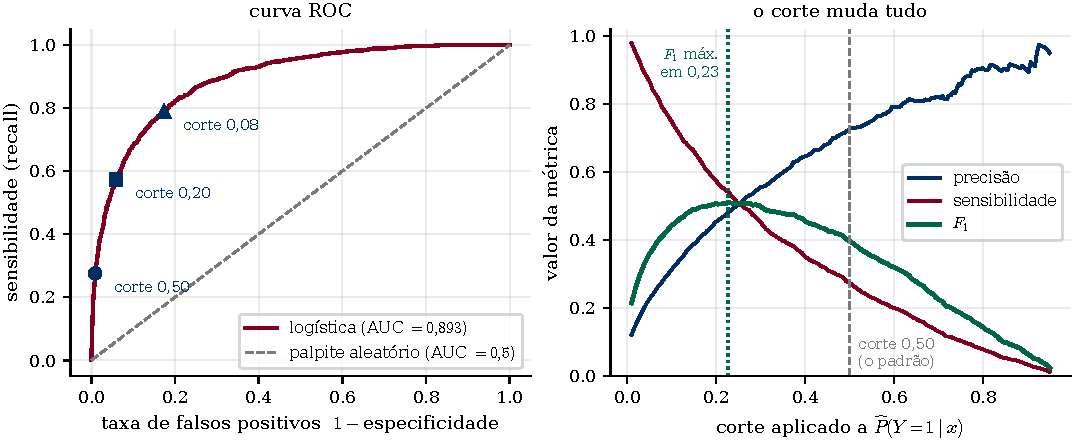
\includegraphics[width=\textwidth]{../../recursos/figuras/08-roc-metricas.pdf}
  \caption{Uma regressão logística ajustada a um problema com prevalência de
  $7{,}9\%$ e avaliada em $20\,000$ observações novas. À esquerda, a curva ROC: cada
  ponto é um corte diferente aplicado ao mesmo modelo. À direita, precisão,
  sensibilidade e $F_1$ em função do corte. No corte padrão, $0{,}50$, a sensibilidade
  é muito baixa, porque poucas observações chegam a essa probabilidade; o $F_1$ é
  máximo perto de $0{,}23$. A acurácia no corte $0{,}50$ é $0{,}935$, contra $0{,}921$
  do classificador que declara todos negativos: o modelo inteiro rende $1{,}4$ ponto
  percentual de acurácia, e a acurácia não é a medida adequada a este problema.}
  \label{fig:roc}
\end{figure}

\begin{ideia}
A curva ROC e a AUC dependem de $\widehat\eta$ apenas pela ordem que ela induz nas
observações: trocar $\widehat\eta$ por qualquer função estritamente crescente dela
deixa a curva igual. Elas servem, portanto, para comparar a capacidade de ordenar de
dois modelos antes de fixar custos. Para escolher o corte, use o da
Proposição~\ref{prop:corte} se os custos forem conhecidos; na falta deles, um critério
comum é maximizar $S+E$, que a Observação~\ref{obs:balanceado} mostrou equivaler a
custos inversamente proporcionais às prevalências.
\end{ideia}

\begin{atencao}
A curva ROC também deve ser estimada numa amostra de teste. Em dados muito
desbalanceados ela pode dar uma impressão otimista, porque a taxa de falsos positivos
divide pelo número de negativos, que é enorme. Mil falsos positivos entre $50\,000$
negativos dão $\text{FPR}=0{,}02$, quase nada no eixo horizontal; mas, se houver $110$
verdadeiros positivos, a precisão é $110/1110\approx0{,}10$, e só um em cada dez
alarmes é verdadeiro. A \emph{curva precisão--revocação}, que traça a precisão contra
a sensibilidade, registra esse custo e informa mais quando os positivos são raros.
\end{atencao}

%==============================================================================
\section{Lidando com dados desbalanceados}\label{sec:desb}
%==============================================================================
Há três estratégias usuais, e as três podem ser lidas como maneiras de codificar
custos.
\begin{description}[leftmargin=2.6cm,style=nextline]
  \item[Mover o corte] Para um classificador que estima $\eta$, basta trocar o corte
        $1/2$ pelo da Proposição~\ref{prop:corte}, ou pela prevalência estimada, como
        na Observação~\ref{obs:balanceado}. O modelo não é reajustado, nenhum dado é
        descartado e as probabilidades estimadas continuam valendo como
        probabilidades.
  \item[Reponderar] Dar peso $w_1$ a cada observação positiva e $w_0$ a cada negativa
        na função objetivo do ajuste (o argumento \texttt{class\_weight} do
        \texttt{scikit-learn}). É a saída natural para métodos que não estimam
        $\eta$; para os que estimam, o efeito é conhecido, e vem a seguir.
  \item[Reamostrar] Alterar a prevalência da amostra de treino, replicando positivos
        (\emph{oversampling}; o SMOTE cria positivos sintéticos por interpolação) ou
        descartando negativos (\emph{undersampling}).
\end{description}

Para um modelo probabilístico ajustado por máxima verossimilhança, como a regressão
logística, o efeito de reponderar pode ser calculado. Para cada $\x$, a
log-verossimilhança ponderada esperada, $w_1\,\eta(\x)\log p+w_0\big(1-\eta(\x)\big)
\log(1-p)$, é máxima em
\[
  p_w(\x)=\frac{w_1\,\eta(\x)}{w_1\,\eta(\x)+w_0\big(1-\eta(\x)\big)}
  \qquad\Longleftrightarrow\qquad
  \frac{p_w(\x)}{1-p_w(\x)}=\frac{w_1}{w_0}\cdot\frac{\eta(\x)}{1-\eta(\x)} ,
\]
como se vê igualando a zero a derivada em $p$. Se o modelo é flexível o bastante para
conter $p_w$, o ajuste reponderado estima $p_w$, e não $\eta$: suas chances ficam
multiplicadas por $w_1/w_0$. (Na regressão logística, se $\eta$ é logística, $p_w$
também é, com o intercepto deslocado de $\log(w_1/w_0)$.) E classificar com
$p_w(\x)>1/2$ é o mesmo que classificar com $\eta(\x)>w_0/(w_0+w_1)$: reponderar
move o corte, mas pelo caminho de distorcer as probabilidades. Com pesos
inversamente proporcionais às frequências de treino, $w_c\propto1/n_c$ (o
\texttt{class\_weight="balanced"}), o corte implícito é $n_1/(n_0+n_1)$, a prevalência
da amostra, exatamente como na Observação~\ref{obs:balanceado}.

Reamostrar tem o mesmo efeito por outro caminho. O modelo é ajustado numa amostra em
que a prevalência é $\pi_1'$, e não $\pi_1$; se a distribuição de $\X$ dentro de cada
classe não muda, o teorema de Bayes diz que as chances que ele estima ficam
multiplicadas por
\[
  \frac{\pi_1'/(1-\pi_1')}{\pi_1/(1-\pi_1)} .
\]
O SMOTE, por criar pontos novos, muda também a distribuição de $\X$ entre os positivos,
e o efeito dele não é exatamente esse.

\begin{atencao}
Reponderar e reamostrar deslocam as probabilidades estimadas por um fator conhecido.
Se você precisa delas como probabilidades da população original, para calcular um
custo esperado ou comunicar um risco, é preciso desfazer esse fator, multiplicando as
chances estimadas pelo seu inverso; mais simples é não mexer no treino e mover o
corte. E não reamostre por reflexo: se os dois erros custam o mesmo, o classificador
de Bayes, com corte $1/2$, já é o correto, por mais desbalanceados que sejam os dados.
\end{atencao}

%==============================================================================
\section{Classificar bem $\neq$ estimar bem probabilidades}\label{sec:calib}
%==============================================================================
Para tomar a decisão, um classificador \emph{plug-in} com corte $K$ só precisa acertar
de que lado do corte está $\eta(\x)$: em todo $\x$ em que $\widehat\eta(\x)-K$ e
$\eta(\x)-K$ têm o mesmo sinal, $g_K$ concorda com o classificador ótimo ([AME] §9.2).
Isso pode acontecer com $\widehat\eta$ muito longe de $\eta$, de modo que classificar
bem não garante estimar bem as probabilidades.

Às vezes, porém, o que se quer são as próprias probabilidades: para ordenar casos por
risco, para calcular o custo esperado de uma decisão quando os custos mudam de caso a
caso, ou para comunicar um risco a alguém. Duas noções interessam então. A primeira é
a \textbf{calibração}: $\widehat\eta$ é calibrada se, entre as observações às quais
atribui probabilidade $p$, a fração de positivos é $p$, isto é,
$\Prob\big(Y=1\mid\widehat\eta(\X)=p\big)=p$. A ferramenta visual correspondente é a
\textbf{curva de calibração}: agrupam-se as observações de teste pela probabilidade
predita e compara-se, em cada grupo, a média predita com a frequência observada de
positivos. Um modelo calibrado fica sobre a diagonal.

A segunda é medir $\widehat\eta$ com uma \textbf{regra de pontuação própria}: uma perda
$s(p,y)$ cujo valor esperado, quando $Y\sim\text{Bernoulli}(\eta)$, é mínimo em
$p=\eta$. As duas mais usadas, estimadas pela média na amostra de teste, são
\begin{itemize}[leftmargin=1.4cm,nosep]
  \item o \textbf{score de Brier}, $s(p,y)=(p-y)^2$, estimado por
        $\frac1m\sum_i\big(\widehat\eta(\X_i)-Y_i\big)^2$;
  \item a \textbf{entropia cruzada} (\emph{log-loss}), a log-verossimilhança negativa
        da Bernoulli, que é o que a regressão logística minimiza:
        $s(p,y)=-\big[\,y\log p+(1-y)\log(1-p)\,\big]$.
\end{itemize}
Para o Brier, a verificação ocupa uma linha: se $Y\sim\text{Bernoulli}(\eta)$,
\[
  \E\big[(p-Y)^2\big]=(p-\eta)^2+\eta\,(1-\eta),
\]
mínimo em $p=\eta$. Tomando a esperança também em $\X$, o risco de Brier de
$\widehat\eta$ é
\[
  \E\big[(\widehat\eta(\X)-Y)^2\big]
  =\E\big[(\widehat\eta(\X)-\eta(\X))^2\big]+\E\big[\eta(\X)\big(1-\eta(\X)\big)\big]:
\]
o erro quadrático de $\widehat\eta$ como estimador de $\eta$, mais uma parcela que não
depende do modelo. É a decomposição da Aula~01 para a regressão, aplicada a
$Y\in\{0,1\}$, cuja função de regressão é $\eta$.

A acurácia e a AUC não são regras próprias. A primeira só vê de que lado do corte
cai cada probabilidade; a segunda só vê a ordem, que não muda quando $\widehat\eta$ é
trocada por qualquer função estritamente crescente dela. Nenhuma das duas registra a
má calibração. Por isso, ao escolher hiperparâmetros por validação cruzada (Aula~03),
use o Brier ou a entropia cruzada quando o que importa são as probabilidades
([AME] §9.2).

\begin{figure}[htbp]
  \centering
  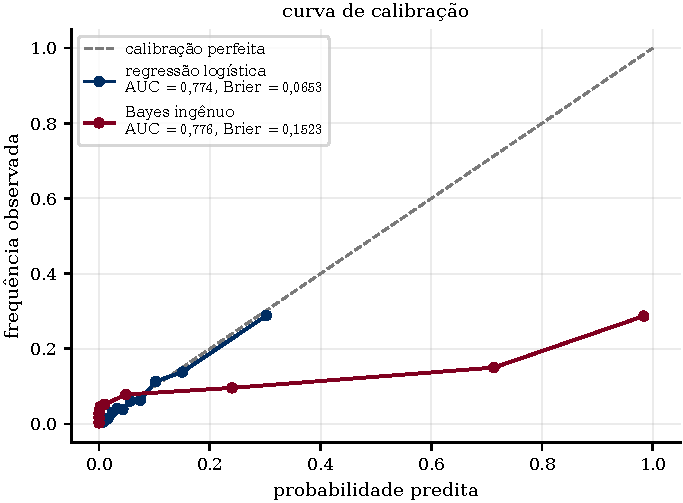
\includegraphics[width=0.62\textwidth]{../../recursos/figuras/08-calibracao.pdf}
  \caption{Curvas de calibração de dois modelos num problema com covariáveis
  fortemente correlacionadas, em que a hipótese do Bayes ingênuo é falsa (prevalência
  de $7{,}9\%$; $20\,000$ observações de teste, agrupadas em dez faixas com o mesmo
  número de observações). Os dois modelos ordenam as observações quase igual, com AUC
  de $0{,}774$ e $0{,}776$, mas o Bayes ingênuo atribui em média $0{,}98$ à faixa mais
  alta, em que só $29\%$ são positivos. O score de Brier ($0{,}065$ para a logística,
  $0{,}152$ para o Bayes ingênuo, mais que o dobro) e a entropia cruzada ($0{,}237$
  contra $0{,}698$) registram a diferença que a AUC não vê.}
  \label{fig:calibracao}
\end{figure}

\begin{ideia}
A Figura~\ref{fig:calibracao} ilustra o título desta seção. Se o objetivo é só
decidir, como aprovar ou não um crédito com um corte escolhido na validação, os dois
modelos servem quase igualmente, e a AUC diz isso corretamente. Se o objetivo é usar
o número, para calcular um custo esperado ou informar um risco, o Bayes ingênuo não
serve, e só uma medida de calibração mostra isso. A métrica deve ser escolhida pela
pergunta que se quer responder.
\end{ideia}

\begin{observacao}
O descalibramento do Bayes ingênuo tem a causa vista na Aula~07: com covariáveis
correlacionadas, o produto $\prod_j f(x_j\mid Y=c)$ conta a mesma evidência várias
vezes, e as probabilidades saem empurradas para $0$ e $1$. Há correções feitas depois
do ajuste: a escala de Platt, que ajusta uma regressão logística sobre os escores, e a
regressão isotônica, que ajusta uma função crescente; o \texttt{scikit-learn} oferece
as duas em \texttt{CalibratedClassifierCV}. Elas precisam de dados próprios, separados
dos usados no ajuste, pelo mesmo motivo de sempre.
\end{observacao}

%==============================================================================
\section*{Resumo}
%==============================================================================
\begin{itemize}[leftmargin=1.4cm]
  \item A acurácia soma os dois erros num número só; numa classe rara, o classificador
        trivial já tem acurácia alta (Fig.~\ref{fig:roc}).
  \item A matriz de confusão (Fig.~\ref{fig:confusao}) estima sensibilidade e
        especificidade, que condicionam na classe verdadeira e não dependem da
        prevalência, e precisão e VPN, que condicionam na decisão e dependem dela; o
        $F_1$ \eqref{eq:f1} é a média harmônica de sensibilidade e precisão. O risco
        $0$--$1$ é a média das taxas de erro das duas classes, ponderada pelas
        prevalências.
  \item Com custos $l_0$ e $l_1$, o corte ótimo é $l_1/(l_0+l_1)$
        (Prop.~\ref{prop:corte}); custos inversamente proporcionais às prevalências
        levam ao corte $\pi_1$ e a maximizar $S+E$.
  \item A curva ROC traça TPR contra FPR à medida que o corte varia; ela e a AUC
        dependem só da ordem dada pelo modelo. Com positivos raros, a curva
        precisão--revocação informa mais.
  \item Mover o corte, reponderar e reamostrar são maneiras de codificar custos; as
        duas últimas deslocam as probabilidades estimadas por um fator conhecido.
  \item Classificar bem não é estimar bem probabilidades (Fig.~\ref{fig:calibracao}):
        para avaliar probabilidades, use a calibração e regras de pontuação próprias,
        como o Brier e a entropia cruzada.
\end{itemize}

\paragraph{Leitura recomendada.} [AME] §7.4 (a matriz de confusão e as medidas
derivadas dela), §9.1 (perdas assimétricas, cortes e dados desbalanceados, de onde vêm
a nossa Prop.~\ref{prop:corte} e a Observação~\ref{obs:balanceado}) e §9.2
(classificação \emph{versus} estimação de probabilidades, o tema da
Figura~\ref{fig:calibracao}). [ISLP] §4.4.2: a matriz de confusão no exemplo do
\texttt{Default}, com uma discussão concreta de sensibilidade numa classe rara, a curva
ROC e a AUC (Figura~4.8), e as Tabelas~4.6 e~4.7, que reúnem os nomes das medidas.

\paragraph{Para praticar.} \texttt{Lista teorica 08.pdf} (teórica, com gabarito) e \texttt{Lista prática 08.ipynb} (prática, para completar as lacunas), nesta mesma pasta.

\end{document}
